%-------------------------------------------------------------------------------
% LATEX TEMPLATE ARTIKEL
%-------------------------------------------------------------------------------
% Dit template is voor gebruik door studenten van de de bacheloropleiding 
% Informatica van de Universiteit van Amsterdam.
% Voor informatie over schrijfvaardigheden, zie 
%                               https://practicumav.nl/schrijven/index.html
%
%-------------------------------------------------------------------------------
%	PACKAGES EN DOCUMENT CONFIGURATIE
%-------------------------------------------------------------------------------

\documentclass{uva-inf-article}
\usepackage[english]{babel}
\usepackage{tikz}
\usepackage{pdflscape}
\usepackage{todonotes}
\usepackage{listings}
\usepackage[demo]{graphicx}
\usepackage{subcaption}
\lstset{
basicstyle=\small\ttfamily,
columns=flexible,
breaklines=true
}

\usepackage[style=authoryear-comp]{biblatex}
\addbibresource{references.bib}

%-------------------------------------------------------------------------------
%	GEGEVENS VOOR IN DE TITEL, HEADER EN FOOTER
%-------------------------------------------------------------------------------

% Geef je artikel een logische titel die de inhoud dekt.
\title{Shogun Live Documentation}

% Vul de naam van de opdracht in zoals gegeven door de docent en het type 
% opdracht, bijvoorbeeld 'technisch rapport' of 'essay'.
% \assignment{}
% \assignmenttype{}

% Vul de volledige namen van alle auteurs in en de corresponderende UvAnetID's.
\authors{Jari Andersen}
% \uvanetids{}

% Vul de naam van je tutor, begeleider (mentor), of docent / vakcoördinator in.
% Vermeld in ieder geval de naam van diegene die het artikel nakijkt!
% \tutor{}
% \mentor{}
% \docent{}

% Vul hier de naam van je tutorgroep, werkgroep, of practicumgroep in.
% \group{SignLab, VisualisationLab}

% Vul de naam van de cursus in en de cursuscode, te vinden op o.a. DataNose.
% \course{}
% \courseid{}

% Dit is de datum die op het document komt te staan. Standaard is dat vandaag.
\date{\today}

%-------------------------------------------------------------------------------
%	VOORPAGINA 
%-------------------------------------------------------------------------------

\begin{document}
\maketitle

%-------------------------------------------------------------------------------
%	INHOUDSOPGAVE EN ABSTRACT
%-------------------------------------------------------------------------------
% Niet toevoegen bij een kort artikel, zeg minder dan 10 pagina's!

%TC:ignore
\tableofcontents
%\begin{abstract}
%\end{abstract}
%TC:endignore
\newpage
%-------------------------------------------------------------------------------
%	INHOUD
%-------------------------------------------------------------------------------
% Hanteer bij benadering IMRAD: Introduction, Method, Results, Discussion.
\section{Introduction}
Welcome to the Shogun Live Documentation! In this guide, we delve into various tools and skills within Shogun Live. Our exploration extends to a range of tools and problems not discussed in the basic tutorials by Vicon.

\section{Best practices and tips}
\subsection{How are markers tracked / how many cameras are needed?}

\subsection{Working with smaller markers and known issues}

\subsubsection{Hemispheres}
1/3 markers or hemisphere markers, are intuitively logical markers to apply onto the fingers. They are low profile making for excellent tactile feel for the actor. However, in our endeavours of trying out various marker sizes, we found hemispheres to be unreliable. When zooming in on the problem by putting a 4mm half marker and a 9mm hemisphere marker in the scene, we can easily see what is going on within the camera view. In figure \ref{fig:hemisphere} we observe the hemisphere on top and the 4mm half marker in the bottom. The camera is viewing the markers from the side. The hemisphere is not recognized as a marker because the blob is not circular like the 4mm marker. But how come the half marker is observed as a circle? The hypothesis is that the 4mm marker is small and the Vero camera's resolution are low, resulting in a blob that is circular. In the Max Planck institute they have further explored this issue by using the Valkery cameras (which have a higher resolution). The Valkery cameras have problems picking up the 4mm half markers due to the same issue as the Vero's picking up the hemispheres.
\begin{figure}[hbt!]
    \centering
    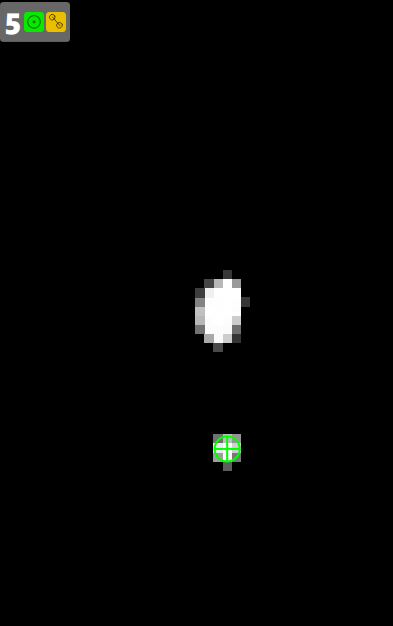
\includegraphics[width=.4\textwidth]{imgs/Hemisphere.png}
    \caption{A comparison between the hemisphere marker (top) and the 4mm marker (bottom) within a camera view. The camera is viewing the markers from the side.}
    \label{fig:hemisphere}
\end{figure}

\subsubsection{Fine tuning the cameras}

\section{Flir}
\url{https://help.vicon.com/space/Shogun112/31235480/Set+up+a+FLIR+Blackfly+S+USB3+video+camera+in+Shogun+Live}

\subsection{Vvid or MOV for the flir}
VVID is the format used for Vicon Video Viewer. In the flir camera setting within Shogun Live, you can switch to MOV if that better suits your purposes.


\section{Bugs and fixes}
In this section we go over various bugs we found and fixes to solve them.

\subsection{Missing retarget in the 3D view}
After creating a retarget in Shogun Post and applying it to the live actor, we came across an issue where we could not visibly see the pink skeleton (retargeted skeleton) in the 3D view. As it turns out the solve was very straightforward. In the processing tab, make sure that the processing output is running at the retarget level.
In addition, also make sure that you have selected the correct actor when adding the retarget.

\subsection{Failed to bind socket acceptor to end point}
When trying to connect to Shogun Live through the Vicon python API we got the following error in the Shogun Live Logs: ``Error ViconCoreAPI Failed to bind socket acceptor to end point. An attempt was made to access a socket in a way forbidden by its access permissions." (figure \ref{fig:socketError}).
This is a Windows issues that can be easily solved by running the commands from the following stackoverflow post \url{https://stackoverflow.com/questions/10461257/an-attempt-was-made-to-access-a-socket-in-a-way-forbidden-by-its-access-permissi}:
\begin{enumerate}
    \item net stop hns
    \item net start hns
\end{enumerate}
Now it should run as smooth as butter again.
\begin{figure}[hbt!]
    \centering
    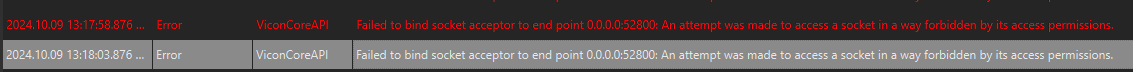
\includegraphics[width=.9\textwidth]{imgs/socketError.png}
    \caption{The ``Error ViconCoreAPI Failed to bind socket acceptor to end point. An attempt was made to access a socket in a way forbidden by its access permissions." error.}
    \label{fig:socketError}
\end{figure}

\subsection{RPC unkown function / callback}
\textit{rpc Unknown: The specified remote function or callback is not known vicon}

Previously, this occurred due to Shogun Live not opening the socket correctly for the client to connect to. Or it was not closed properly? I'm not sure, but I fixed it by closing Shogun Live and then opening it again. If that doesn't fix it, then close Shogun Live and open it again (doing it three times fixed it for me for some reason).

Don't forget, this error can also come from Shogun Post. So make sure to restart this as well.

Lastly, I have also been lucky opening Shogun Post/Live as administrator to fix this issue.

\subsection{Why am I not seeing FLIR video / FLIR is blackscreen / triggerGPOWarning}
When encountering a blackscreen on the FLIR with the trigger GPO warning (see figure \ref{fig:triggerGPOWarning}), make sure to select the correct Trigger GPO option in the property window of the FLIR camera (see figure \ref{fig:triggerGPO}). It should match the port to which the FLIR camera is connected to the Vicon Lock.
\begin{figure}[hbt!]
    \centering
    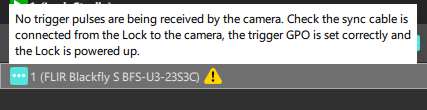
\includegraphics[width=.5\textwidth]{imgs/triggerGPOWarning.png}
    \caption{The Trigger GPO Warning.}
    \label{fig:triggerGPOWarning}
\end{figure}
\begin{figure}[hbt!]
    \centering
    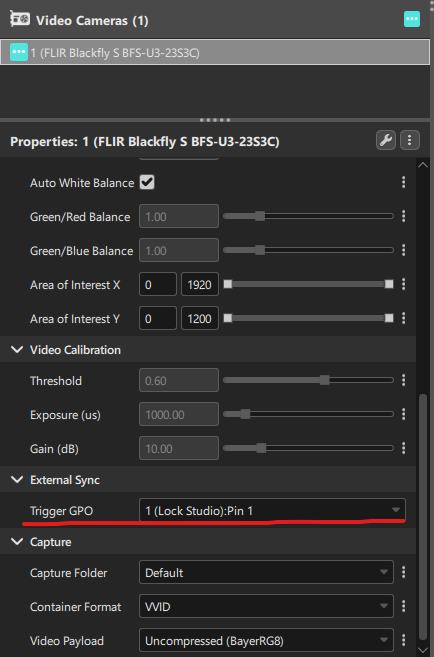
\includegraphics[width=.5\textwidth]{imgs/triggerGPO.png}
    \caption{The Trigger GPO option.}
    \label{fig:triggerGPO}
\end{figure}


\subsection{Gray cameras / Not contributing, gray play icon}
When a camera is not contributing (grayed out, gray play icon), that is usually due to the amount of noise coming into the camera. Sadly, you will not see the noise in the camera view because it is not contributing. They way we solved this issue in the past is by simply turning the diaphragm down for the cameras that have this issue. When refocusing a camera, make sure that in addition to putting markers in the scene, you also stand in the scene with some semi-reflective clothing in order to see if all cameras are contributing.
%-------------------------------------------------------------------------------
%	REFERENTIES
%-------------------------------------------------------------------------------

\printbibliography

%-------------------------------------------------------------------------------
%	BIJLAGEN 
%-------------------------------------------------------------------------------

%TC:ignore
% \appendix 
% \section{Bijlage {\LaTeX} code}
% Bijgevoegd zijn de \textattachfile{main.tex}{code} en 
% \textattachfile{references.bib}{bibliografie}.
%TC:endignore

%-------------------------------------------------------------------------------
\end{document}